\documentclass[11pt,a4paper]{cibb}

% Fallback definition for missing \@ordinalM
\makeatletter
\providecommand{\@ordinalM}[2]{#1}
\makeatother

\usepackage{subfigure,graphicx}
\usepackage{amsmath,amsfonts,latexsym,amssymb,euscript,xr}
\usepackage{booktabs}
\usepackage[nodayofweek]{datetime}
\usepackage{hyperref}
\usepackage{fmtcount}
\usepackage[english]{datenumber}
\usepackage[absolute]{textpos}

\usepackage[table]{xcolor}
\usepackage{color,colortbl,tabularx}

\usepackage[english]{babel}
\usepackage[protrusion=true,expansion=true]{microtype}
\usepackage{amsmath,amsfonts,amsthm}
\usepackage{pifont}
\usepackage{tikz}
\usetikzlibrary{positioning,arrows.meta}

\def\red{\color{red}}
\def\black{\color{black}}
\def\blue{\color{blue}}
\def\magenta{\color{magenta}}

\definecolor{LightBlue}{rgb}{0.88,0.9,0.9}

\newcommand\blfootnote[1]{%
  \begingroup
  \renewcommand\thefootnote{}\footnote{#1}%
  \addtocounter{footnote}{-1}%
  \endgroup
}

\title{\Large $\ $\\ \bf Phone-Watch Contrastive Representation Learning for Subject-Generalized Wearable Activity Recognition}

\author{\blue \large Krishna Mula$^1$, Yash Khairnar$^{1}$}
\address{\blue \footnotesize $\ $\\$^1$ Computer Science Department, San Jose State University. \\
%
%
% \bigskip
% ORCID codes: FA 0000-0000-0000-0000; SA 0000-0000-0000-0000; TA 0000-0000-0000-0000.
% \bigskip
% \newline
% $^*$corresponding author: email@email.com
% \bigskip
% \newline
% [The initial submission must be anonymous.
% Do not edit the blue text sections of this short paper template before the initial submission.
% Include information about author names and affiliations, conflict of interests, acknowledgments, data and software availability, and funding in black text only in the resubmission.]
}

\abstract{\small wearable sensing, human activity recognition, contrastive learning, multimodal fusion, subject generalization. \normalsize
\\[17pt]
{\bf Abstract} We study activity recognition from synchronized phone and watch inertial streams under a subject-disjoint evaluation protocol.
The dataset provides per-subject files for phone and watch accelerometer and gyroscope recordings, with activity labels stored as contiguous letter-coded segments.
We build a segment-aware preprocessing pipeline that pairs the four streams by activity episode, resamples them onto a shared 20\,Hz timeline, and writes normalized 3\,s windows with 1\,s stride, yielding 50,091 training, 12,744 validation, and 47,790 test windows as $(12, 60)$ tensors.

We compare five tiers of learning: (i) classical models (Decision Tree, Gaussian NB, Linear SVM, Random Forest, AdaBoost, XGBoost) trained on 84-dimensional handcrafted feature vectors; (ii) supervised 1D CNN, ANN, and LSTM baselines trained on fused, watch-only, and phone-only raw windows; (iii) a phone-watch contrastive model that learns paired embeddings via symmetric InfoNCE loss, evaluated through frozen linear probes; (iv) a comprehensive architecture comparison across CNN, ANN, and LSTM; and (v) transfer learning from UCI HAR with systematic layer freezing and progressive unfreezing.

The best deep model from the full sweep is the supervised watch-only CNN baseline at 64.47\% accuracy and 0.6471 macro F1, followed by LSTM (61.27\%, 0.6117) and ANN (59.42\%, 0.5930).
The strongest contrastive result remains the watch-only frozen probe at 58.31\% accuracy and 0.5777 macro F1.
We also explore transfer learning from UCI HAR and observe \textbf{negative transfer}: every fine-tuning strategy underperforms the from-scratch baseline (CNN frozen: 51.26\%, LSTM frozen: 35.04\%), likely because the domain gap between UCI HAR's six generic activities and our 18 fine-grained classes is too large for direct feature reuse.

A consistent finding across all architectures is strong device asymmetry: watch-only models substantially outperform phone-only and fusion variants regardless of architecture, suggesting that wrist motion carries most of the discriminative signal and that current phone-watch fusion is not yet robust enough to exploit both devices effectively.
}

\begin{document}

\renewcommand{\thefootnote}{}
\footnotetext{\small{Article version: \datedate $\;$ h\currenttime  $\;$ CET}}

\thispagestyle{myheadings}
\pagestyle{myheadings}

\section{Introduction}
\label{sec:SCIENTIFIC-BACKGROUND}

Human activity recognition from wearables is a natural test bed for representation learning: labels are expensive, while unlabeled sensor streams are plentiful.
This project focuses on a phone-watch setting in which two devices observe the same activity from different body locations.

The working hypothesis is that synchronized phone and watch windows provide complementary views of the same underlying motion pattern.
Aligning those views during pretraining should yield representations that transfer better to unseen subjects and under limited labels.

This report has two goals: to document a reliable preprocessing and windowing pipeline for the four sensor streams, and to compare watch-first supervised baselines against cross-view contrastive pretraining followed by frozen linear probes.

\section{Literature Review}
\label{sec:LITERATURE-REVIEW}

Recent advances in human activity recognition (HAR) have increasingly leveraged self-supervised and contrastive learning to address challenges of label scarcity and domain variability in wearable sensor data. A key direction is learning invariant representations across different sensor configurations. For instance, contrastive representation learning across sensor locations demonstrates that contrastive objectives can effectively transfer knowledge between sensor placements, making it highly relevant to cross-device scenarios such as smartphone--smartwatch alignment~\cite{placeholder_contrastive_sensor_locations}. Complementing this, large-scale studies like self-supervised learning for HAR using 700,000 person-days of wearable data provide strong empirical evidence that self-supervised pretraining significantly improves generalization and label efficiency, establishing a foundation for scalable HAR systems~\cite{placeholder_ssl_700k}. Methodologically, works such as temporal contrastive learning for sensor-based HAR~\cite{placeholder_temporal_contrastive} and TS-TCC~\cite{placeholder_tstcc} highlight the effectiveness of temporal and contextual contrasting in capturing meaningful time-series dynamics, while TS2Vec~\cite{placeholder_ts2vec} extends this idea toward learning universal time-series representations applicable across tasks and domains. Beyond single-device settings, MM-HAR~\cite{placeholder_mmhar} emphasizes the importance of multimodal learning using consumer wearables, reinforcing the need to handle heterogeneous sensor inputs. Additionally, applications in healthcare, such as wearable-based contrastive learning for clinical monitoring~\cite{placeholder_clinical_monitoring}, further validate the robustness of these approaches in real-world deployments. Traditional deep learning surveys on wearable HAR~\cite{placeholder_dl_survey_har} provide essential context regarding datasets, benchmarks, and challenges, while recent self-supervised HAR works~\cite{placeholder_ssl_har_generalization,placeholder_ssl_har_reduced_labels} underline improvements in cross-dataset generalization and reduced dependence on labeled data. Together, these studies motivate the use of contrastive self-supervised learning as a principled approach for learning device-invariant representations, particularly for cross-location and cross-device HAR scenarios.

\subsection{Comparative Summary}

Table~\ref{tab:lit-review} synthesizes the ten surveyed papers across five dimensions: key ideas, models, datasets, metrics, and limitations.

\begin{table}[htb!] \scriptsize
\centering
    \begin{tabularx}{\textwidth}{ l  X  X  X  X  X }
        \toprule
        \textbf{Paper} & \textbf{Key Ideas} & \textbf{Models} & \textbf{Datasets} & \textbf{Metrics} & \textbf{Limitations} \\
        \midrule
        \rowcolor{LightBlue} Contrastive across locations~\cite{placeholder_contrastive_sensor_locations} & Cross-sensor alignment via contrastive loss & CNN encoder, InfoNCE & Wearable IMU (multiple placements) & Accuracy, F1, AUC & Limited to controlled placements \\
        SSL 700K days~\cite{placeholder_ssl_700k} & Large-scale self-supervised pretraining on unlabeled wearables & Transformer, SimCLR & 700K person-days consumer wearables & Accuracy, calibration & Compute-intensive; consumer-grade noise \\
        \rowcolor{LightBlue} Temporal contrastive HAR~\cite{placeholder_temporal_contrastive} & Temporal context prediction for sensor data & LSTM, GRU, CPC & Opportunity, PAMAP2, UCI-HAR & Accuracy, F1, per-class metrics & Requires long contiguous windows \\
        TS-TCC~\cite{placeholder_tstcc} & Temporal-spectral contrastive coding & CNN, Transformer & UEA multivariate archive & Accuracy, F1 & Hyperparameter-sensitive to augmentation strength \\
        \rowcolor{LightBlue} TS2Vec~\cite{placeholder_ts2vec} & Universal time-series representations via hierarchical contrastive learning & Dilated CNN & 125 UCR/UEA datasets & Accuracy, AUC & Generalizes across tasks but task-agnostic \\
        MM-HAR~\cite{placeholder_mmhar} & Multimodal fusion of phone and watch IMU & CNN-LSTM, attention & Self-collected phone+watch dataset & Accuracy, F1, confusion matrices & Small cohort; limited cross-subject validation \\
        \rowcolor{LightBlue} Clinical contrastive~\cite{placeholder_clinical_monitoring} & Self-supervised pretraining for clinical wearable monitoring & CNN, SimCLR & Hospital ICU wearables & AUC-ROC, sensitivity & Domain-specific; limited generalization \\
        DL survey HAR~\cite{placeholder_dl_survey_har} & Comprehensive review of deep learning for wearable HAR & CNN, RNN, LSTM, attention & 20+ public HAR datasets & Accuracy, F1, AUC, inference cost & Focus on supervised; limited SSL coverage \\
        \rowcolor{LightBlue} SSL cross-dataset~\cite{placeholder_ssl_har_generalization} & Cross-dataset generalization via self-supervised pretraining & CNN, MoCo & Four public HAR datasets & Cross-dataset accuracy & Performance degrades with dataset shift \\
        SSL reduced labels~\cite{placeholder_ssl_har_reduced_labels} & Reducing label dependence through self-supervision & CNN, SimCLR & UCI-HAR, WISDM & Accuracy @ 1\%, 5\%, 10\% labels & Marginal gains at very low label budgets \\
        \bottomrule
    \end{tabularx}
    \caption{\textbf{Literature review comparative summary.}
    All ten surveyed papers address wearable sensor data and activity recognition, with a clear trend toward contrastive and self-supervised learning as a means to reduce annotation cost and improve cross-subject generalization.
    \label{tab:lit-review}}
\end{table}

The surveyed literature reveals three consistent themes: (i)~self-supervised and contrastive objectives are increasingly standard for reducing label dependence in wearable HAR; (ii)~multimodal fusion of phone and watch remains challenging, with most gains coming from single-device (especially wrist) representations; and (iii)~cross-subject generalization is the primary open problem, motivating the subject-disjoint evaluation protocol adopted in this project.

\section{Dataset Exploration}
\label{sec:DATA}

\subsection{Raw Dataset Structure}

The raw data are organized into subject-disjoint \texttt{train/} and \texttt{test/} folders, each containing four sensor collections: \texttt{phone/accel}, \texttt{phone/gyro}, \texttt{watch/accel}, and \texttt{watch/gyro}.
Every file covers one subject and one stream; each row contains \texttt{subject\_id}, an activity label, a timestamp, and three sensor axes.
Labels are exposed as letter codes rather than human-readable activity names.

The cached window manifest contains 18 activity codes: A, B, C, D, E, F, G, H, I, J, K, L, M, O, P, Q, R, and S.
All per-class analysis in this draft uses those codes directly, as the semantic mapping is not yet stored in the repository.

\subsection{Split Summary}

The raw paired-segment index contains 628 candidate activity episodes; 625 have all four required streams and 3 are dropped due to missing phone accelerometer and gyroscope data.

After preprocessing, we obtain the subject-disjoint split in Table~\ref{tab:split-summary}.
Validation subjects are deterministically carved from the raw training subjects, ensuring no leakage across splits.

\begin{table}[httb!] \small
\centering
    \begin{tabularx}{0.9\textwidth}{ l  c  c  X }
        \toprule
        \textbf{Split} & \textbf{\# Subjects} & \textbf{\# Windows} & \textbf{Notes} \\
        \midrule
        \rowcolor{LightBlue} Train & 16 & 50,091 & Used for supervised fitting and contrastive pretraining. \\
        Val   & 4  & 12,744 & Held out from training subjects for model selection. \\
        \rowcolor{LightBlue} Test  & 14 & 47,790 & Unseen subjects only; subject 1629 contributes a second activity occurrence per class. \\
        \bottomrule
    \end{tabularx}
    \caption{\textbf{Window cache summary.}
    Cached windows under \texttt{artifacts/windows/} are the source of truth for all experiments.
    \label{tab:split-summary}}
\end{table}

The split is close to class-balanced: validation and test have 708 and 2,655 windows per class, respectively.
Training is nearly balanced, with small deficits for B, F, J, and O due to the three removed episodes.

\subsection{Dataset Summary}

\begin{table}[htb!] \small
\centering
    \begin{tabularx}{0.96\textwidth}{ l  c  X }
        \toprule
        \textbf{Statistic} & \textbf{Value} & \textbf{Notes} \\
        \midrule
        \rowcolor{LightBlue} Participants & 34 & 20 raw training subjects and 14 raw test subjects. \\
        Raw files & 136 & One file per subject-device-stream combination. \\
        \rowcolor{LightBlue} Input streams & 4 & Phone accelerometer, phone gyroscope, watch accelerometer, and watch gyroscope. \\
        Activity codes & 18 & Letter-coded labels A--S, excluding N. \\
        \rowcolor{LightBlue} Raw sensor rows & 9,841,341 & Sum across all inertial files before segment pairing and windowing. \\
        Days per participant & not directly observable & Each participant contributes exactly one raw file per stream in one split, which suggests one recording session per participant, but the timestamps are not linked to calendar dates. \\
        \rowcolor{LightBlue} Demographic metadata & unavailable & No age or gender fields appear in the shared dataset files. \\
        \bottomrule
    \end{tabularx}
    \caption{\textbf{Raw dataset summary.}
    This table addresses the metadata items directly observable from the released files.
    \label{tab:raw-summary}}
\end{table}

\begin{table}[htb!] \scriptsize
\centering
    \begin{tabular}{ c  r  c  r  c  r }
        \toprule
        \textbf{Label} & \textbf{Rows} & \textbf{Label} & \textbf{Rows} & \textbf{Label} & \textbf{Rows} \\
        \midrule
        A & 555,095 & B & 532,870 & C & 538,369 \\
        D & 546,977 & E & 558,964 & F & 530,915 \\
        G & 549,077 & H & 544,383 & I & 546,991 \\
        J & 531,125 & K & 568,730 & L & 542,065 \\
        M & 553,721 & O & 540,826 & P & 551,872 \\
        Q & 552,736 & R & 547,014 & S & 549,611 \\
        \bottomrule
    \end{tabular}
    \caption{\textbf{Raw sensor rows per activity code.}
    Counts are nearly balanced even before window extraction, ranging from 530,915 (F) to 568,730 (K).
    \label{tab:raw-label-counts}}
\end{table}

\section{Annotation and Signal Exploration}

Each file is an ordered concatenation of contiguous activity episodes rather than one continuous recording, and the same label can appear multiple times for one subject.
We therefore index episodes by \texttt{(subject\_id, activity\_label, occurrence\_index)} rather than by absolute timestamp.
This segment-aware view is the key design choice that keeps phone-watch alignment faithful to the annotation structure.

Figure~\ref{fig:label-timeline} illustrates the annotation structure directly.
For subject 1600, both phone and watch accelerometer streams show long contiguous runs with synchronized A$\rightarrow$B$\rightarrow$C transitions.
This justifies treating activity labels as episode-level segments rather than isolated frame-wise events.

\begin{figure}[htb!]
  \centering
  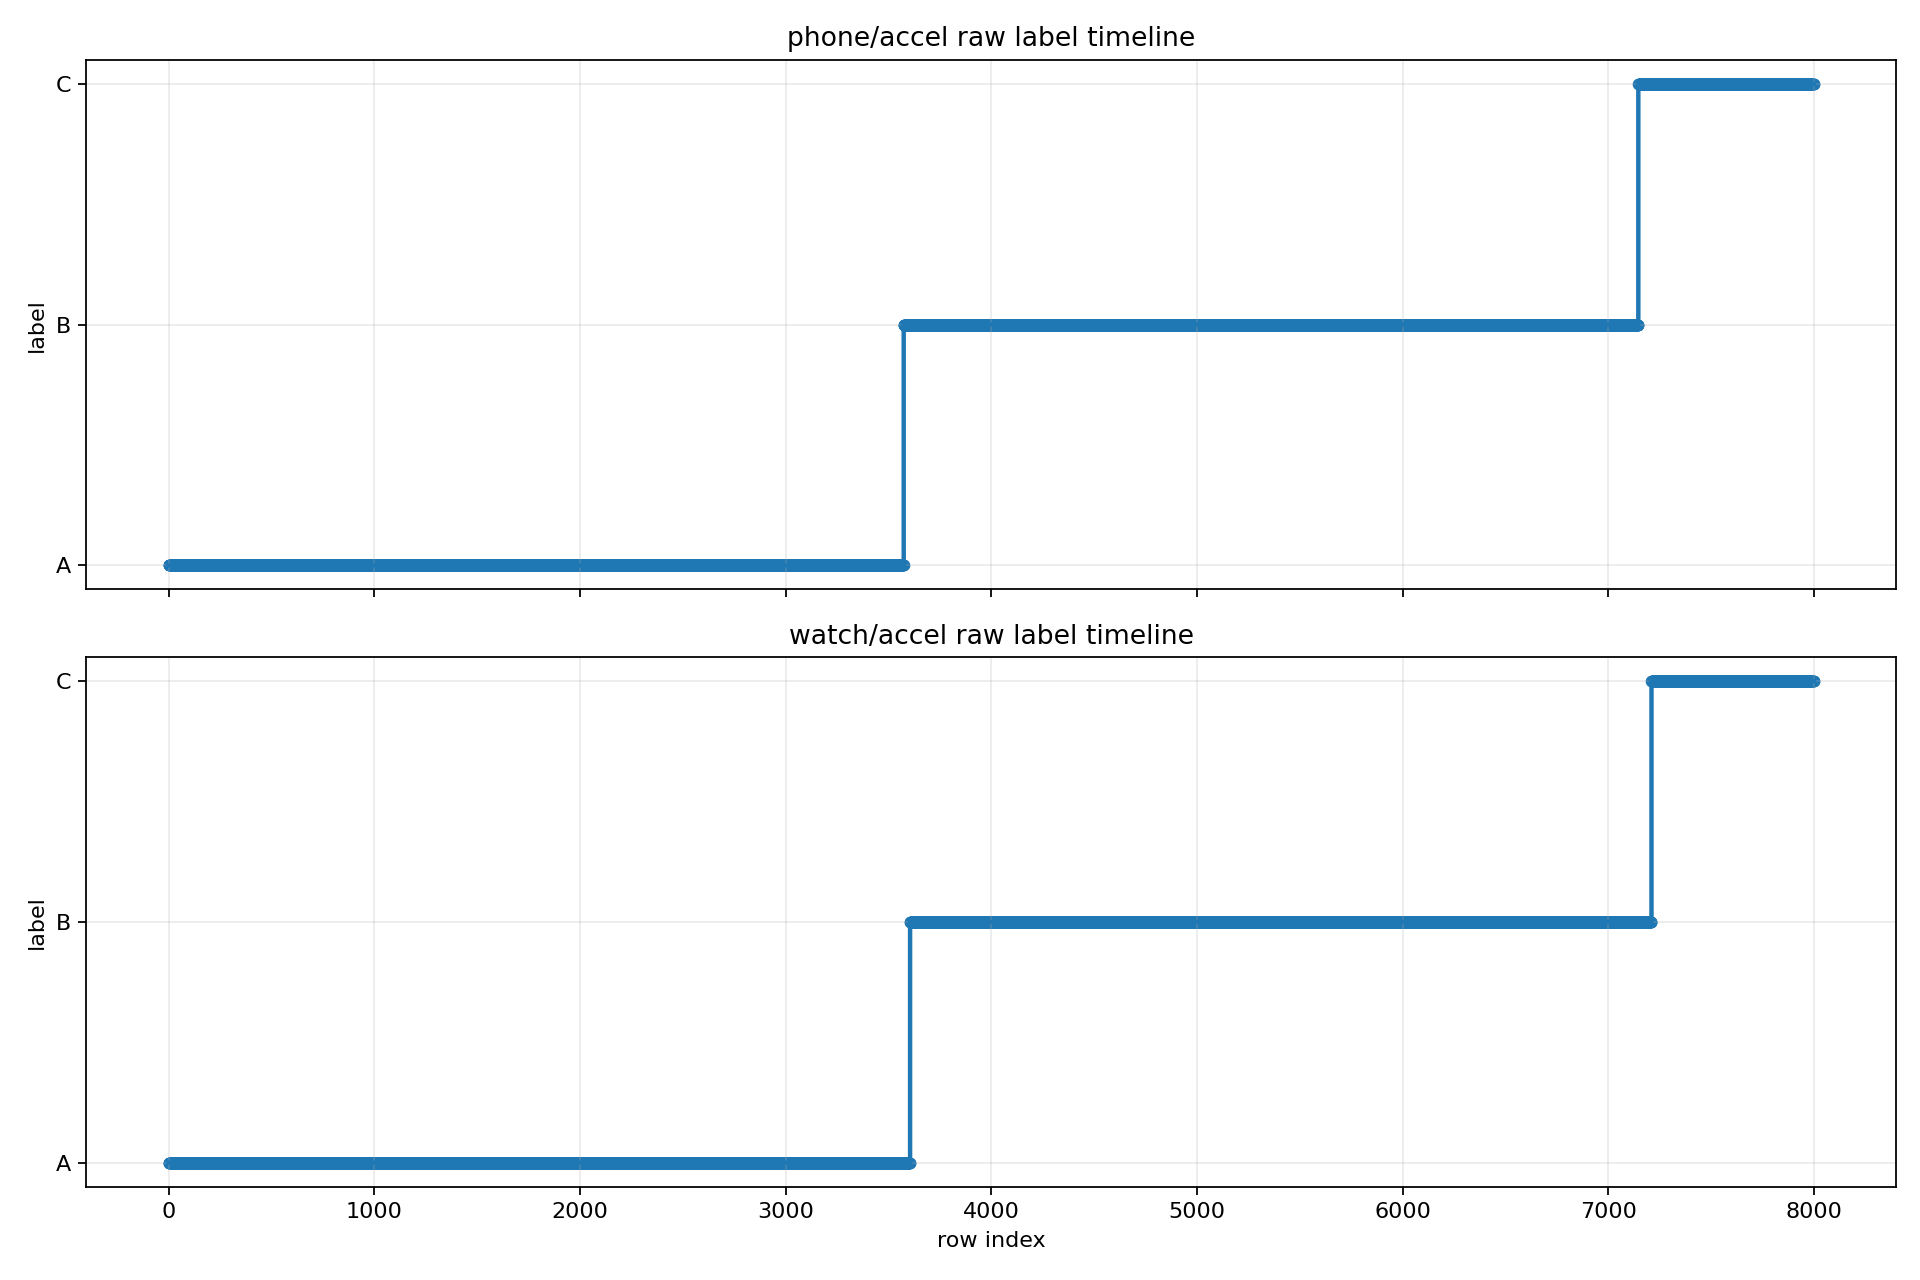
\includegraphics[width=0.92\linewidth]{figures/subject_1600_A0_label_timeline.png}
  \caption{\textbf{Raw label timeline around labeled activity events (subject 1600).}
  The first 8,000 rows of the phone and watch accelerometer streams exhibit matching contiguous label blocks, including clear A$\rightarrow$B$\rightarrow$C transitions.}
  \label{fig:label-timeline}
\end{figure}

Valid paired episodes are highly regular, with a mean overlapping duration of approximately 179.71\,s and very small spread across subjects and classes.
With a 3\,s window and 1\,s stride, each standard episode yields 177 windows.

Native sampling rates differ across streams: phone accelerometer averages 25.55\,Hz, phone gyroscope 21.14\,Hz, and both watch streams approximately 20.79\,Hz.
This heterogeneity makes direct sample-by-sample fusion inappropriate without resampling.

Figure~\ref{fig:signal-walkthrough} shows one representative paired segment for subject 1600, activity A.
The top panel gives the raw phone/watch $x$-axis traces over the episode, and the bottom panel shows the selected 3\,s window after interpolation to the shared 20\,Hz grid.

\begin{figure}[htb!]
  \centering
  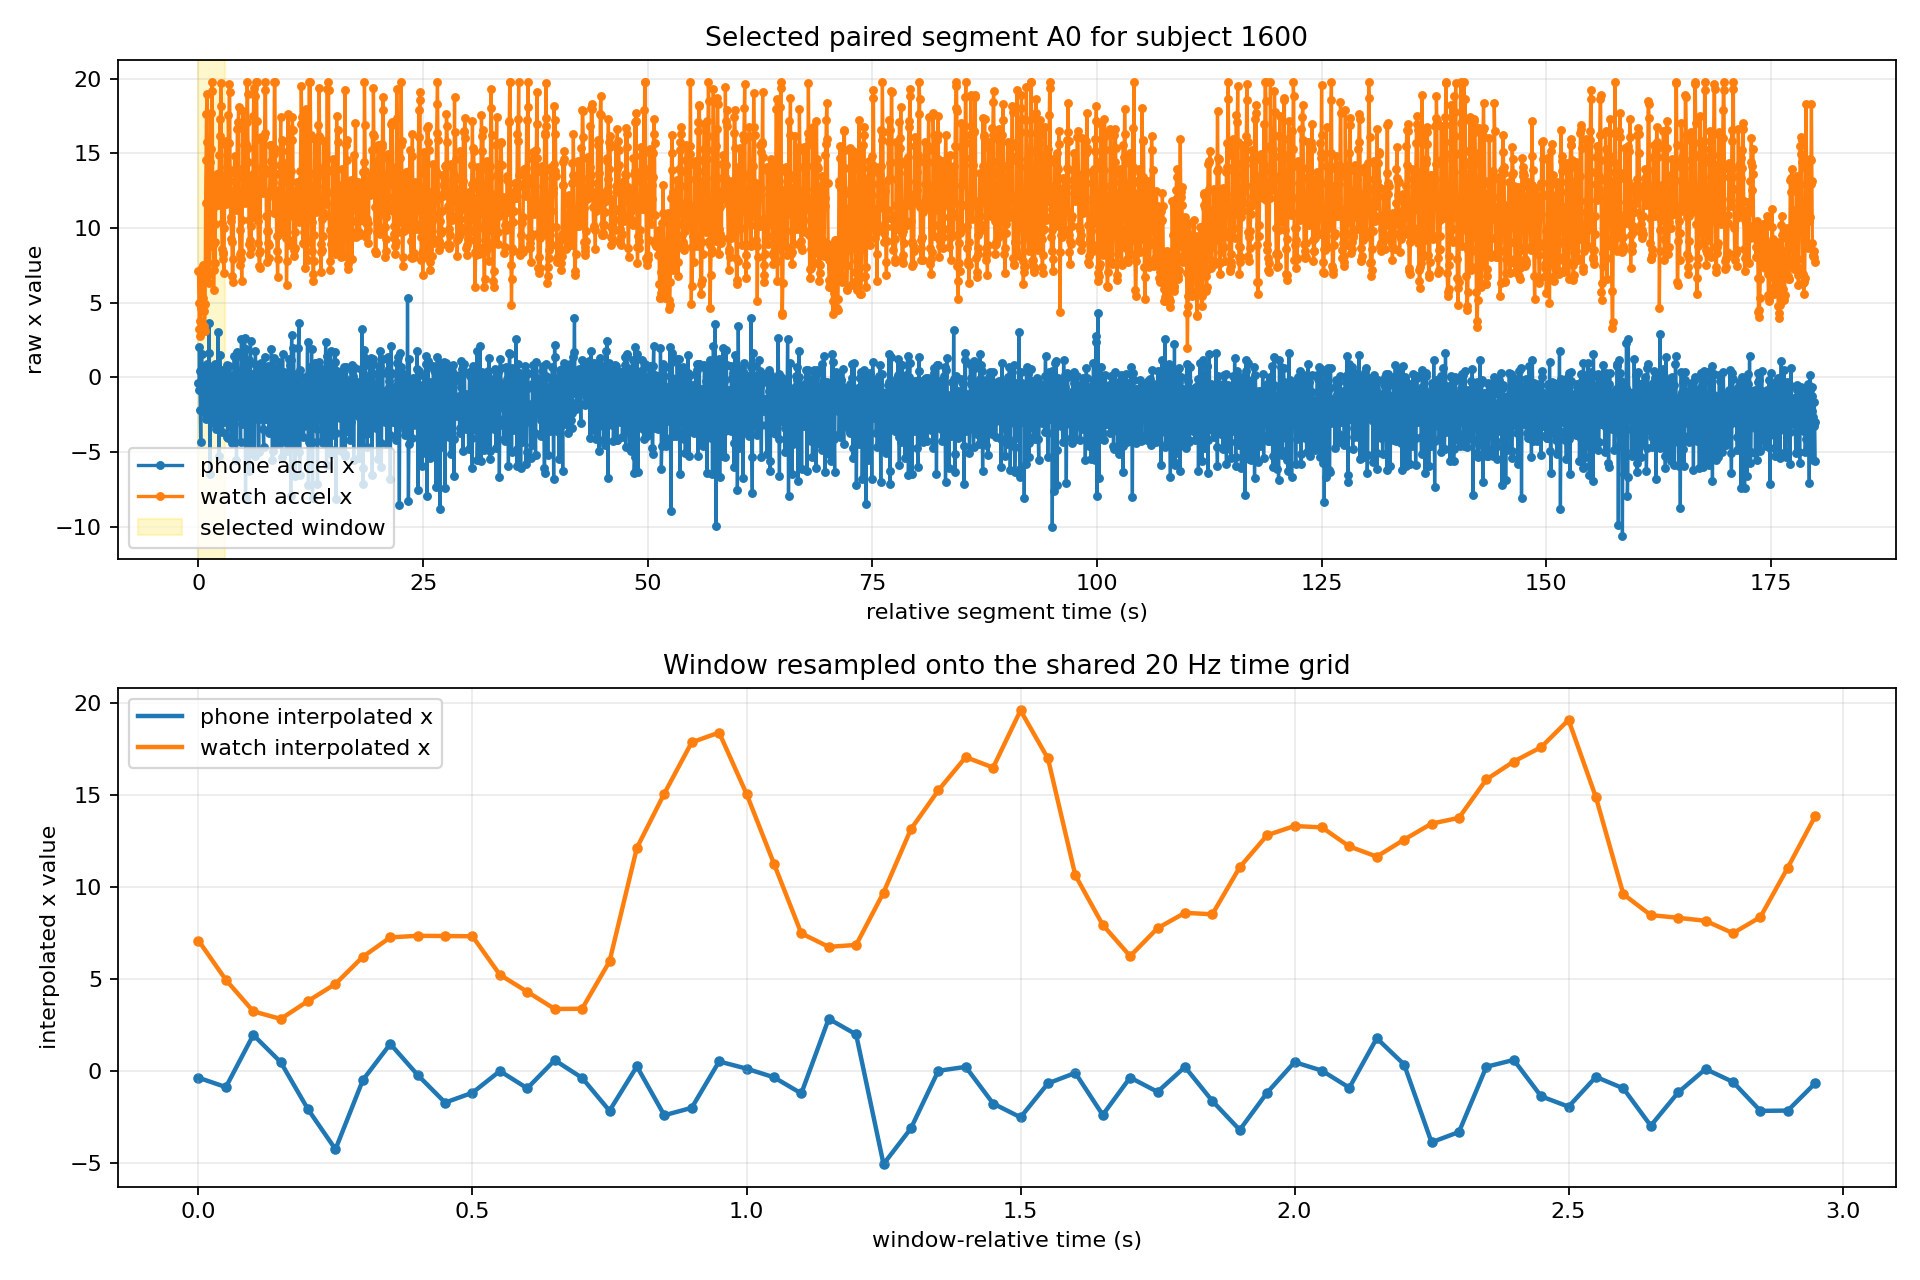
\includegraphics[width=0.92\linewidth]{figures/raw_to_resampled_walkthrough.png}
  \caption{\textbf{Raw-to-resampled signal walkthrough (subject 1600, activity A).}
  The highlighted region in the raw segment becomes one 3\,s analysis window after interpolation onto the shared 20\,Hz timeline.
  This figure serves both as signal exploration and as a before/after preprocessing comparison.}
  \label{fig:signal-walkthrough}
\end{figure}

\section{Signal Preprocessing}

The preprocessing pipeline parses each stream into contiguous runs of the same activity code; each run becomes one candidate segment with start row, end row, duration, and native sampling-rate metadata.

Four-stream episode pairs are built by matching segments with the same activity code and occurrence index.
Only episodes containing all four streams (phone accelerometer, phone gyroscope, watch accelerometer, and watch gyroscope) are kept.

Within each valid episode, we compute the common overlapping duration across the four streams and operate on relative time within that overlap.
Each sensor axis is linearly interpolated onto a shared 20\,Hz grid.
The final fused tensor stacks streams in a fixed order and produces a normalized $(12, 60)$ window.
Channel-wise z-score statistics are estimated on the training windows and stored in \texttt{artifacts/windows/manifest.json}.

No additional low-pass or handcrafted denoising filter is applied in the current artifact set.
This is a deliberate scope choice: the present report isolates the value of segment-aware alignment, interpolation, and normalization before introducing heavier preprocessing.

\section{Windowing Strategies}

Each window spans 3.0\,s with a 1.0\,s stride, yielding 60 samples after resampling.
Window centers range from 1.5\,s to 177.5\,s within a standard episode.
Because windows are generated after segment pairing, every window belongs to a single activity episode and never crosses label transitions---labels are inherited from the paired episode, and all cached windows are aligned across phone and watch.

For label-efficiency experiments, the 10\% subset is selected deterministically within each \texttt{(subject, class)} bucket, keeping at least one example per bucket when possible.
This ensures that the 10\% supervised baseline and the 10\% probe use comparable labeled subsets.

\section{Feature Extraction \& Analysis}

\subsection{Handcrafted Features for Classical Baselines}

We extract an 84-dimensional feature vector from each normalized $(12, 60)$ window.
The 12 channels are ordered as phone accelerometer ($x,y,z$), phone gyroscope ($x,y,z$), watch accelerometer ($x,y,z$), and watch gyroscope ($x,y,z$).
For each channel we compute four time-domain and three frequency-domain statistics, giving $12 \times 7 = 84$ features per window.

\textbf{Time-domain} (4 per channel): mean, standard deviation, root mean square (RMS), and zero-crossing rate (ZCR).

\textbf{Frequency-domain} (3 per channel): dominant frequency (Hz, from the peak of the one-sided FFT magnitude, excluding DC), spectral energy ($\sum |F_k|^2 / N$), and spectral entropy ($-\sum p_k \log_2 p_k$, where $p_k$ is the normalized power spectrum).

Figure~\ref{fig:rf-importance} shows the top-20 features ranked by Random Forest impurity importance.
Watch accelerometer channels dominate, consistent with the watch-over-phone advantage observed across all model tiers.

\begin{figure}[htb!]
  \centering
  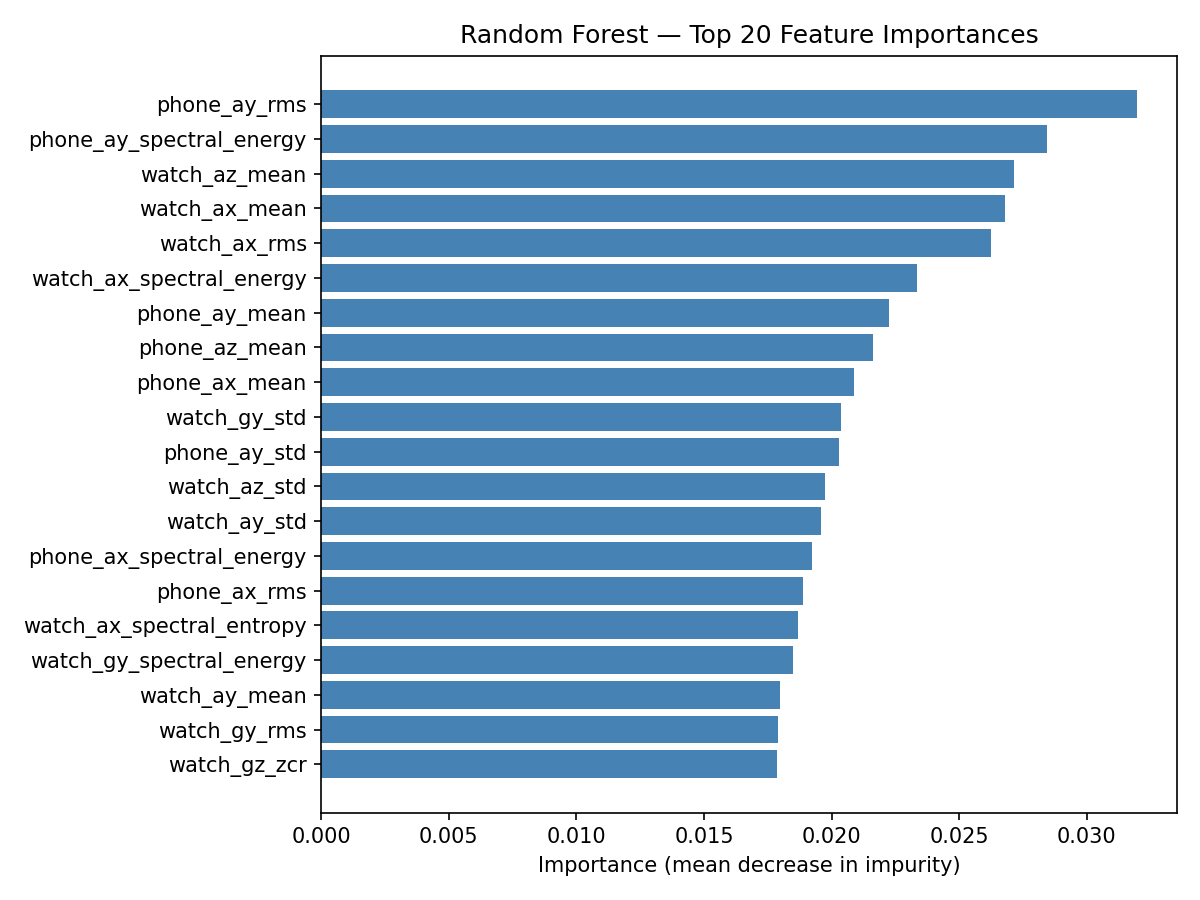
\includegraphics[width=0.85\linewidth]{figures/rf_feature_importance.png}
  \caption{\textbf{Top-20 feature importances from Random Forest.}
  Watch accelerometer features rank highest, corroborating the device asymmetry finding.}
  \label{fig:rf-importance}
\end{figure}

\subsection{Learned Representations}

The supervised baseline uses a 1D CNN encoder (\texttt{TimeSeriesEncoder}) with three temporal convolution blocks, batch normalization, ReLU activations, and max pooling, followed by global average pooling.
The encoder outputs a 256-dimensional feature vector; a linear classifier maps it to one of the 18 activity codes.
Figure~\ref{fig:cnn-arch} shows the full architecture.

\begin{figure}[htb!]
\centering
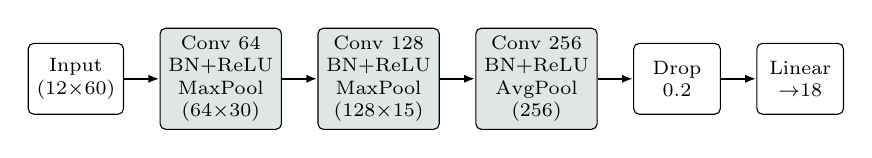
\begin{tikzpicture}[
  box/.style={draw, rounded corners=2pt, minimum width=1.45cm, minimum height=0.9cm,
              align=center, font=\scriptsize, fill=LightBlue, inner sep=3pt},
  sml/.style={draw, rounded corners=2pt, minimum width=1.1cm,  minimum height=0.9cm,
              align=center, font=\scriptsize, fill=white, inner sep=3pt},
  arr/.style={-{Latex[length=4pt]}, thick},
  node distance=0.45cm
]
  \node[sml] (in)   {Input\\$(12{\times}60)$};
  \node[box,  right=of in]  (c1) {Conv 64\\BN+ReLU\\MaxPool\\$(64{\times}30)$};
  \node[box,  right=of c1]  (c2) {Conv 128\\BN+ReLU\\MaxPool\\$(128{\times}15)$};
  \node[box,  right=of c2]  (c3) {Conv 256\\BN+ReLU\\AvgPool\\$(256)$};
  \node[sml,  right=of c3]  (dp) {Drop\\$0.2$};
  \node[sml,  right=of dp]  (cl) {Linear\\${\to}18$};
  \foreach \a/\b in {in/c1, c1/c2, c2/c3, c3/dp, dp/cl}
    \draw[arr] (\a) -- (\b);
\end{tikzpicture}
\caption{\textbf{Supervised HAR model.}
The \texttt{TimeSeriesEncoder} backbone (three Conv1D blocks) is shared across all supervised
and contrastive variants. Input channels are 12 for fusion mode, 6 for phone-only or watch-only.}
\label{fig:cnn-arch}
\end{figure}

\subsubsection{ANN Baseline}

The fully-connected baseline flattens each normalized $(C, 60)$ window into a $C \times 60$ vector and passes it through a two-layer MLP with ReLU activations and dropout:
\begin{itemize}
    \item Flatten: $(C, 60) \to C \times 60$ (720-D for fusion, 360-D for single-device)
    \item Linear$(C \times 60, 512)$, ReLU, Dropout$(0.2)$
    \item Linear$(512, 256)$, ReLU, Dropout$(0.2)$
    \item Linear$(256, 18)$
\end{itemize}
This architecture tests whether raw-window flattening plus a deep MLP can match or exceed the temporal models.

\subsubsection{LSTM Baseline}

The recurrent baseline treats each window as a sequence of 60 time steps with $C$ channels per step:
\begin{itemize}
    \item Permute: $(B, C, T) \to (B, T, C)$
    \item 2-layer LSTM with hidden size 128, batch-first, dropout$(0.2)$
    \item Mean-pooling over the time dimension
    \item Linear$(128, 18)$
\end{itemize}
The LSTM is expected to capture temporal ordering better than the ANN, while the CNN's local receptive fields and subsampling may offer a complementary inductive bias for motion-pattern classification.

The contrastive model uses separate phone and watch encoders with the same backbone, each consuming a $(6, 60)$ view and producing a 256-dimensional representation.
Projection heads reduce embeddings from 256 to 128 to 64 dimensions before the symmetric InfoNCE loss is applied.
Figure~\ref{fig:contrastive-arch} illustrates the full pretraining setup and how the frozen encoder outputs are reused for linear probing.

\begin{figure}[htb!]
\centering
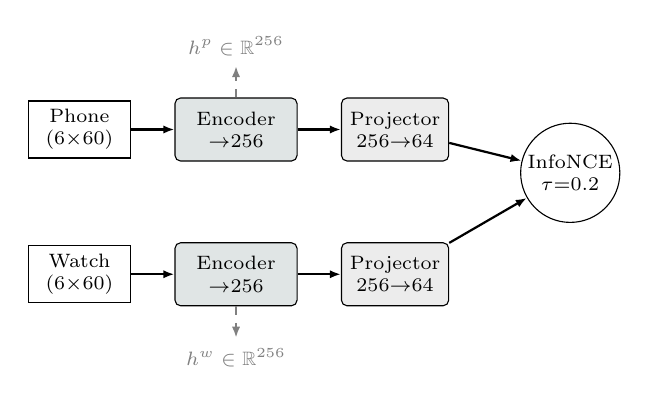
\begin{tikzpicture}[
  inp/.style={draw, minimum width=1.3cm, minimum height=0.7cm,
              align=center, font=\scriptsize, inner sep=3pt},
  enc/.style={draw, rounded corners=2pt, minimum width=1.55cm, minimum height=0.8cm,
              align=center, font=\scriptsize, fill=LightBlue, inner sep=3pt},
  prj/.style={draw, rounded corners=2pt, minimum width=1.35cm, minimum height=0.8cm,
              align=center, font=\scriptsize, fill=gray!15, inner sep=3pt},
  lss/.style={draw, circle, minimum size=1.1cm, align=center, font=\scriptsize,
              fill=white, inner sep=1pt},
  arr/.style={-{Latex[length=4pt]}, thick},
  node distance=0.5cm and 0.55cm
]
  %% Phone path (top row)
  \node[inp] (xp) {Phone\\$(6{\times}60)$};
  \node[enc, right=of xp] (ep) {Encoder\\${\to}256$};
  \node[prj, right=of ep] (pp) {Projector\\$256{\to}64$};

  %% Watch path (bottom row, aligned under phone)
  \node[inp, below=1.1cm of xp] (xw) {Watch\\$(6{\times}60)$};
  \node[enc, right=of xw]       (ew) {Encoder\\${\to}256$};
  \node[prj, right=of ew]       (pw) {Projector\\$256{\to}64$};

  %% InfoNCE node centred between the two projection outputs
  \node[lss, right=0.9cm of pp, yshift=-0.55cm] (L) {InfoNCE\\$\tau{=}0.2$};

  %% Main arrows
  \draw[arr] (xp) -- (ep);  \draw[arr] (ep) -- (pp);  \draw[arr] (pp) -- (L);
  \draw[arr] (xw) -- (ew);  \draw[arr] (ew) -- (pw);  \draw[arr] (pw) -- (L);

  %% Frozen-probe annotation on the encoder outputs
  \draw[arr,dashed,gray] (ep.north) -- ++(0,0.4)
        node[above,font=\scriptsize,gray]{$h^p \in \mathbb{R}^{256}$};
  \draw[arr,dashed,gray] (ew.south) -- ++(0,-0.4)
        node[below,font=\scriptsize,gray]{$h^w \in \mathbb{R}^{256}$};
\end{tikzpicture}
\caption{\textbf{Contrastive pretraining architecture.}
Phone and watch views pass through separately parameterised encoders with the same backbone.
After pretraining the encoders are frozen; $h^p$ and $h^w$ (dashed) are concatenated into a
512-D vector for the paired linear probe, or used individually for single-device probes.}
\label{fig:contrastive-arch}
\end{figure}

For downstream evaluation, the paired probe concatenates frozen $h^p$ and $h^w$ into a 512-dimensional feature vector fed to a linear head.
Single-device probes use only $h^p$ or $h^w$, isolating each device's contribution.

\section{Modeling and Results}

\subsection{Classical Machine Learning}

We train six classical models on the 84-dimensional handcrafted features: Decision Tree (max depth 20), Gaussian Naive Bayes, Random Forest (200 trees), Linear SVM with Platt calibration, AdaBoost (100 estimators), and XGBoost (200 trees, histogram method).
All models are evaluated on the subject-disjoint test set---a more stringent protocol than random 80/20 or 70/30 splits, since test subjects are completely unseen during training.
Table~\ref{tab:classical-results} reports macro precision, macro recall, accuracy, macro F1, and macro one-vs-rest AUC.

\begin{table}[htb!] \scriptsize
\centering
    \begin{tabularx}{0.98\textwidth}{ l  c  c  c  c  c }
        \toprule
        \textbf{Method} & \textbf{Prec.} & \textbf{Recall} & \textbf{Acc.} & \textbf{Macro F1} & \textbf{Macro AUC} \\
        \midrule
        \rowcolor{LightBlue} Decision Tree       & 0.4331 & 0.4099 & 0.4099 & 0.4088 & 0.6934 \\
        Gaussian NB              & 0.5580 & 0.5447 & 0.5447 & 0.5354 & 0.8985 \\
        \rowcolor{LightBlue} Linear SVM           & 0.5971 & 0.5833 & 0.5833 & 0.5662 & 0.9255 \\
        Random Forest            & 0.6221 & 0.6021 & 0.6021 & 0.5838 & 0.9503 \\
        \rowcolor{LightBlue} AdaBoost             & 0.3999 & 0.3554 & 0.3554 & 0.3058 & 0.8894 \\
        Hist.\ Grad.\ Boost      & 0.5877 & 0.5727 & 0.5727 & 0.5549 & 0.9140 \\
        \bottomrule
    \end{tabularx}
    \caption{\textbf{Classical ML results on the subject-disjoint test set.}
    Because the test split is perfectly class-balanced, macro recall numerically matches accuracy to four decimals.
    Random Forest achieves the best accuracy (60.2\%) and macro AUC (0.950).
    \label{tab:classical-results}}
\end{table}

Figure~\ref{fig:rf-confusion} shows the confusion matrix of the strongest classical model, Random Forest.
Its diagonal is sharp for classes B, O, P, Q, and S, while confusion remains concentrated among the harder mid-performing classes such as D, F, H, I, J, K, and L.
This error pattern is broadly consistent with the deep-model analysis later in the report.

\begin{figure}[htb!]
  \centering
  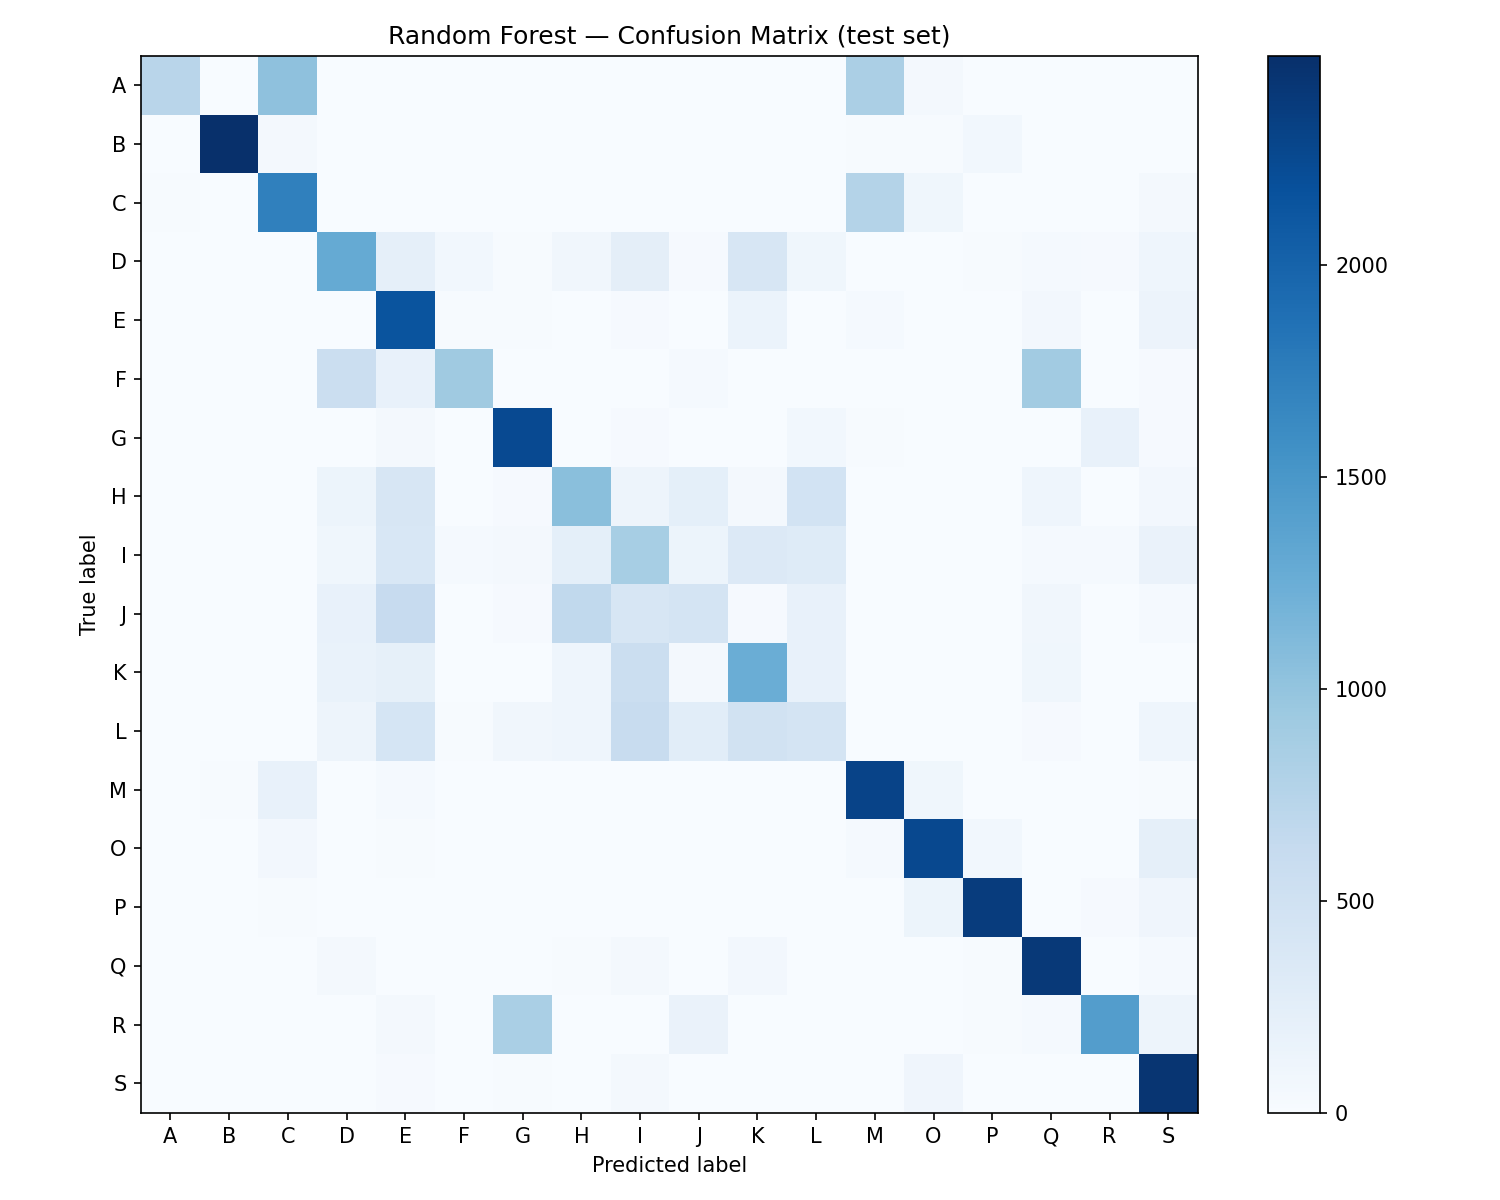
\includegraphics[width=0.78\linewidth]{figures/rf_confusion_matrix.png}
  \caption{\textbf{Random Forest confusion matrix on the subject-disjoint test set.}
  The strongest classical baseline shows clean separation for several classes but still struggles on the same ambiguous activity groups seen in the deep models.}
  \label{fig:rf-confusion}
\end{figure}

\subsection{Supervised and Contrastive Setup}

The supervised baseline is trained end-to-end with cross-entropy loss using AdamW (learning rate $10^{-3}$, weight decay $10^{-4}$, batch size 256, dropout 0.2) with early stopping on validation macro F1.

Contrastive pretraining uses training windows without labels.
Phone and watch views are augmented with Gaussian jitter, mild amplitude scaling, and short temporal masking before being passed through the dual encoders.
The pretraining objective is symmetric InfoNCE with in-batch negatives and temperature $\tau = 0.2$:
\begin{equation}
\mathcal{L} =
\frac{1}{2N}
\sum_{i=1}^{N}
\left[
- \log \frac{\exp(\mathrm{sim}(z_i^p, z_i^w)/\tau)}{\sum_{j=1}^{N}\exp(\mathrm{sim}(z_i^p, z_j^w)/\tau)}
- \log \frac{\exp(\mathrm{sim}(z_i^w, z_i^p)/\tau)}{\sum_{j=1}^{N}\exp(\mathrm{sim}(z_i^w, z_j^p)/\tau)}
\right].
\label{eq:infonce}
\end{equation}

After pretraining, encoder weights are frozen and linear heads are trained for paired, phone-only, and watch-only probes at 10\% and 100\% label fractions.

\subsection{Evaluation Protocol}

All headline numbers are reported on the held-out test subjects.
We track macro precision, macro recall, accuracy, macro F1, per-class F1, per-subject accuracy, confusion matrices, and ROC/AUC when probability outputs are available.
Because the cached test split is exactly balanced at 2,655 windows per class, macro recall numerically equals overall accuracy in the tables below.
The demo rubric mentions conventional random 80/20 or 70/30 splits, but we instead report the stricter subject-disjoint protocol because unseen-subject generalization is the central project goal.
The primary benchmark is now the watch-only supervised baseline, because it is the strongest simple model under subject-disjoint evaluation.
Contrastive probes are therefore judged against the watch baseline first and against the weaker fusion and phone baselines second.

\section{Results}
\label{sec:RESULTS}

\subsection{Deep Learning Architecture Comparison}

Table~\ref{tab:full-sweep} presents the complete CNN/ANN/LSTM sweep across all three channel modes.
The best overall result is the watch-only CNN at 0.6447 accuracy and 0.6471 macro F1, followed by LSTM (0.6127, 0.6117) and ANN (0.5942, 0.5930).

\begin{table}[httb!] \scriptsize
\centering
    \begin{tabularx}{0.98\textwidth}{ l  l  c  c  c }
        \toprule
        \textbf{Model} & \textbf{Channel} & \textbf{Test Acc.} & \textbf{Macro F1} & \textbf{Best Epoch} \\
        \midrule
        \rowcolor{LightBlue} CNN   & watch  & \textbf{0.6447} & \textbf{0.6471} & 36 \\
        LSTM  & watch  & 0.6127 & 0.6117 & 22 \\
        \rowcolor{LightBlue} ANN   & watch  & 0.5942 & 0.5930 & 39 \\
        CNN   & fusion & 0.5001 & 0.4937 & 1 \\
        \rowcolor{LightBlue} LSTM  & fusion & 0.3805 & 0.3692 & 2 \\
        ANN   & fusion & 0.3874 & 0.3819 & 3 \\
        \rowcolor{LightBlue} CNN   & phone  & 0.1817 & 0.1740 & 16 \\
        LSTM  & phone  & 0.1945 & 0.1878 & 4 \\
        \rowcolor{LightBlue} ANN   & phone  & 0.1807 & 0.1805 & 14 \\
        \bottomrule
    \end{tabularx}
    \caption{\textbf{Full architecture sweep results on the subject-disjoint test set.}
    CNN consistently outperforms LSTM and ANN on watch, while all architectures fail on phone and underperform on fusion.
    The test split is exactly class-balanced (2,655 windows per class), so accuracy equals macro recall.
    \label{tab:full-sweep}}
\end{table}

Figure~\ref{fig:model-comparison} visualizes the same hierarchy: watch-only bars dominate, fusion is intermediate, and phone is near chance for all three architectures.

\begin{figure}[htb!]
  \centering
  \includegraphics[width=0.92\linewidth]{drive-download-figures/fig1_model_comparison_bars.png}
  \caption{\textbf{Model comparison across architectures and channels.}
  CNN achieves the best watch-only performance; all architectures degrade sharply on phone and fusion inputs.}
  \label{fig:model-comparison}
\end{figure}

\subsection{Transfer Learning from UCI HAR}

A natural extension of the supervised and contrastive baselines is to leverage an external, larger HAR corpus for encoder pretraining and then fine-tune on the target dataset.
We choose the UCI Human Activity Recognition (UCI HAR) dataset as the pretraining source because it is widely used, well-documented, and contains raw tri-axial inertial signals that are temporally compatible with our windows.

\subsubsection{Pretraining Corpus}

UCI HAR contains six daily activities (walking, walking upstairs, walking downstairs, sitting, standing, laying) recorded from 30 subjects with a waist-mounted smartphone at 50\,Hz.
The released raw inertial signals (not the 561 pre-processed feature vectors) are segmented into 128-sample windows with 50\% overlap, giving $(6, 128)$ tensors per window.
Because our encoder uses adaptive average pooling before the classifier, it is length-agnostic: both 128-sample (UCI HAR) and 60-sample (our dataset) windows map to the same 256-dimensional embedding, so no architectural surgery is required.

We pretrain separate CNN and LSTM encoders on UCI HAR for 40 epochs with AdamW ($\mathrm{lr}=10^{-3}$, weight decay $10^{-4}$, batch size 256) and early stopping on validation accuracy.
After pretraining, encoder weights are saved and transferred to our dataset.

\subsubsection{Fine-tuning Protocol}

All transfer experiments use watch-only input (the strongest channel mode from Section~\ref{sec:RESULTS}) and are trained for up to 40 epochs with a reduced learning rate of $10^{-4}$ (one tenth of the scratch baseline) to avoid catastrophic forgetting of pretrained features.
We investigate four layer-freezing strategies:

\begin{itemize}
    \item \textbf{Scratch (none)}: Train the full model from random initialization; serves as the transfer-learning baseline.
    \item \textbf{Frozen (all)}: Freeze the entire pretrained encoder; only the linear classifier head is trained.
    \item \textbf{Partial (first\_two)}: Freeze the first two convolutional or LSTM blocks and fine-tune only the final block plus the classifier.
    \item \textbf{Progressive}: Start with a fully frozen encoder and unfreeze all encoder parameters at epoch 10.
    When unfreezing occurs, both the optimizer and the learning-rate scheduler are recreated to prevent momentum desync and to apply the lower fine-tuning LR to the newly trainable parameters.
\end{itemize}

\subsubsection{Transfer Learning Results}

Table~\ref{tab:transfer-results} reports test accuracy and macro F1 for all eight configurations.
Figure~\ref{fig:transfer-accuracy} visualizes the same results as grouped bars, and Figure~\ref{fig:transfer-curves} shows the validation macro-F1 learning curves with vertical annotations at the progressive unfreeze epoch.

\begin{table}[htb!] \scriptsize
\centering
    \begin{tabular}{l l c c}
        \toprule
        \textbf{Model} & \textbf{Freeze Strategy} & \textbf{Test Acc.} & \textbf{Macro F1} \\
        \midrule
        CNN  & Scratch (none)               & 0.6452 & 0.6465 \\
        CNN  & Frozen (all)                 & 0.5126 & 0.4888 \\
        CNN  & Partial (first two)          & 0.5877 & 0.5811 \\
        CNN  & Progressive (unfreeze @ 10)  & 0.5820 & 0.5649 \\
        \midrule
        LSTM & Scratch (none)               & 0.6127 & 0.6117 \\
        LSTM & Frozen (all)                 & 0.3504 & 0.3135 \\
        LSTM & Partial (first two)          & 0.4753 & 0.4606 \\
        LSTM & Progressive (unfreeze @ 10)  & 0.4294 & 0.3903 \\
        \bottomrule
    \end{tabular}
    \caption{\textbf{Transfer learning results on the subject-disjoint test set.}
    All models use watch-only input. Pretraining corpus: UCI HAR (6 activities, 30 subjects).
    Negative transfer is observed: every fine-tuning strategy underperforms the from-scratch baseline.
    \label{tab:transfer-results}}
\end{table}

\begin{figure}[htb!]
  \centering
  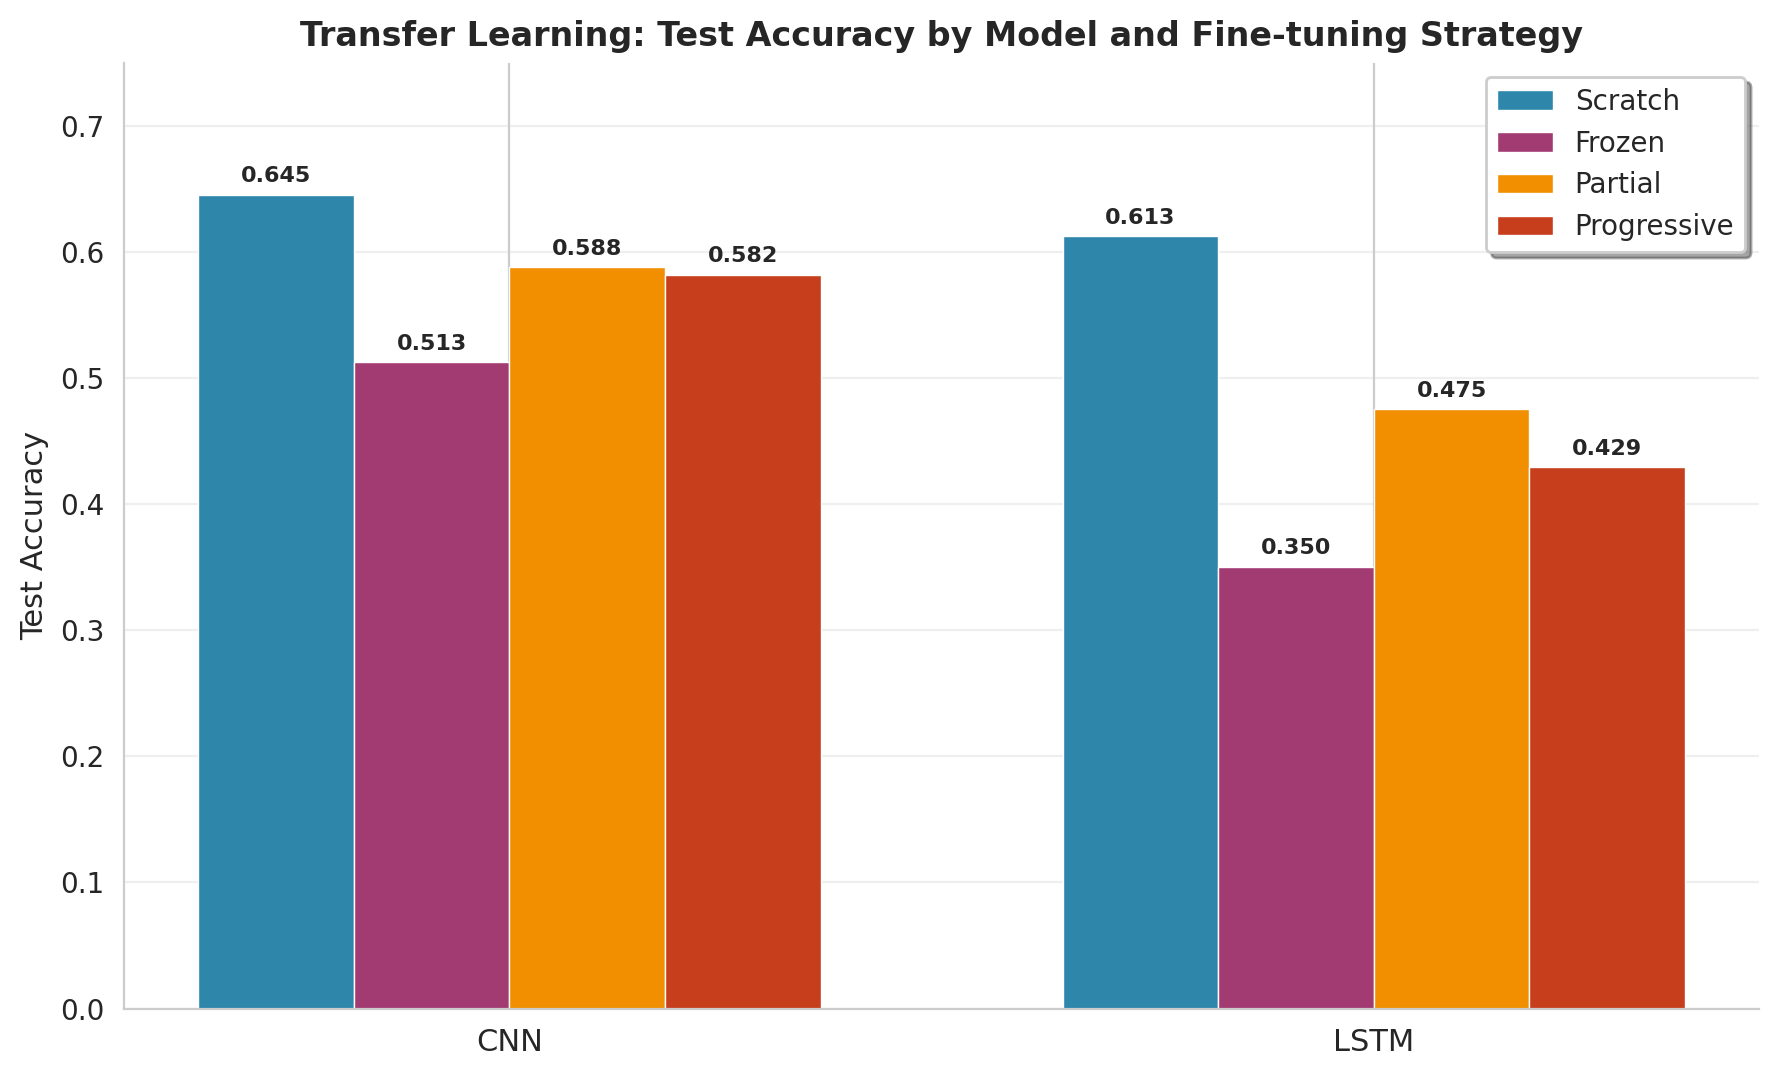
\includegraphics[width=0.92\linewidth]{figures/fig_transfer_accuracy.png}
  \caption{\textbf{Transfer learning test accuracy by model and fine-tuning strategy.}
  Every pretrained variant underperforms the corresponding scratch baseline; the gap is largest for the fully frozen encoder.
  \label{fig:transfer-accuracy}}
\end{figure}

\begin{figure}[htb!]
  \centering
  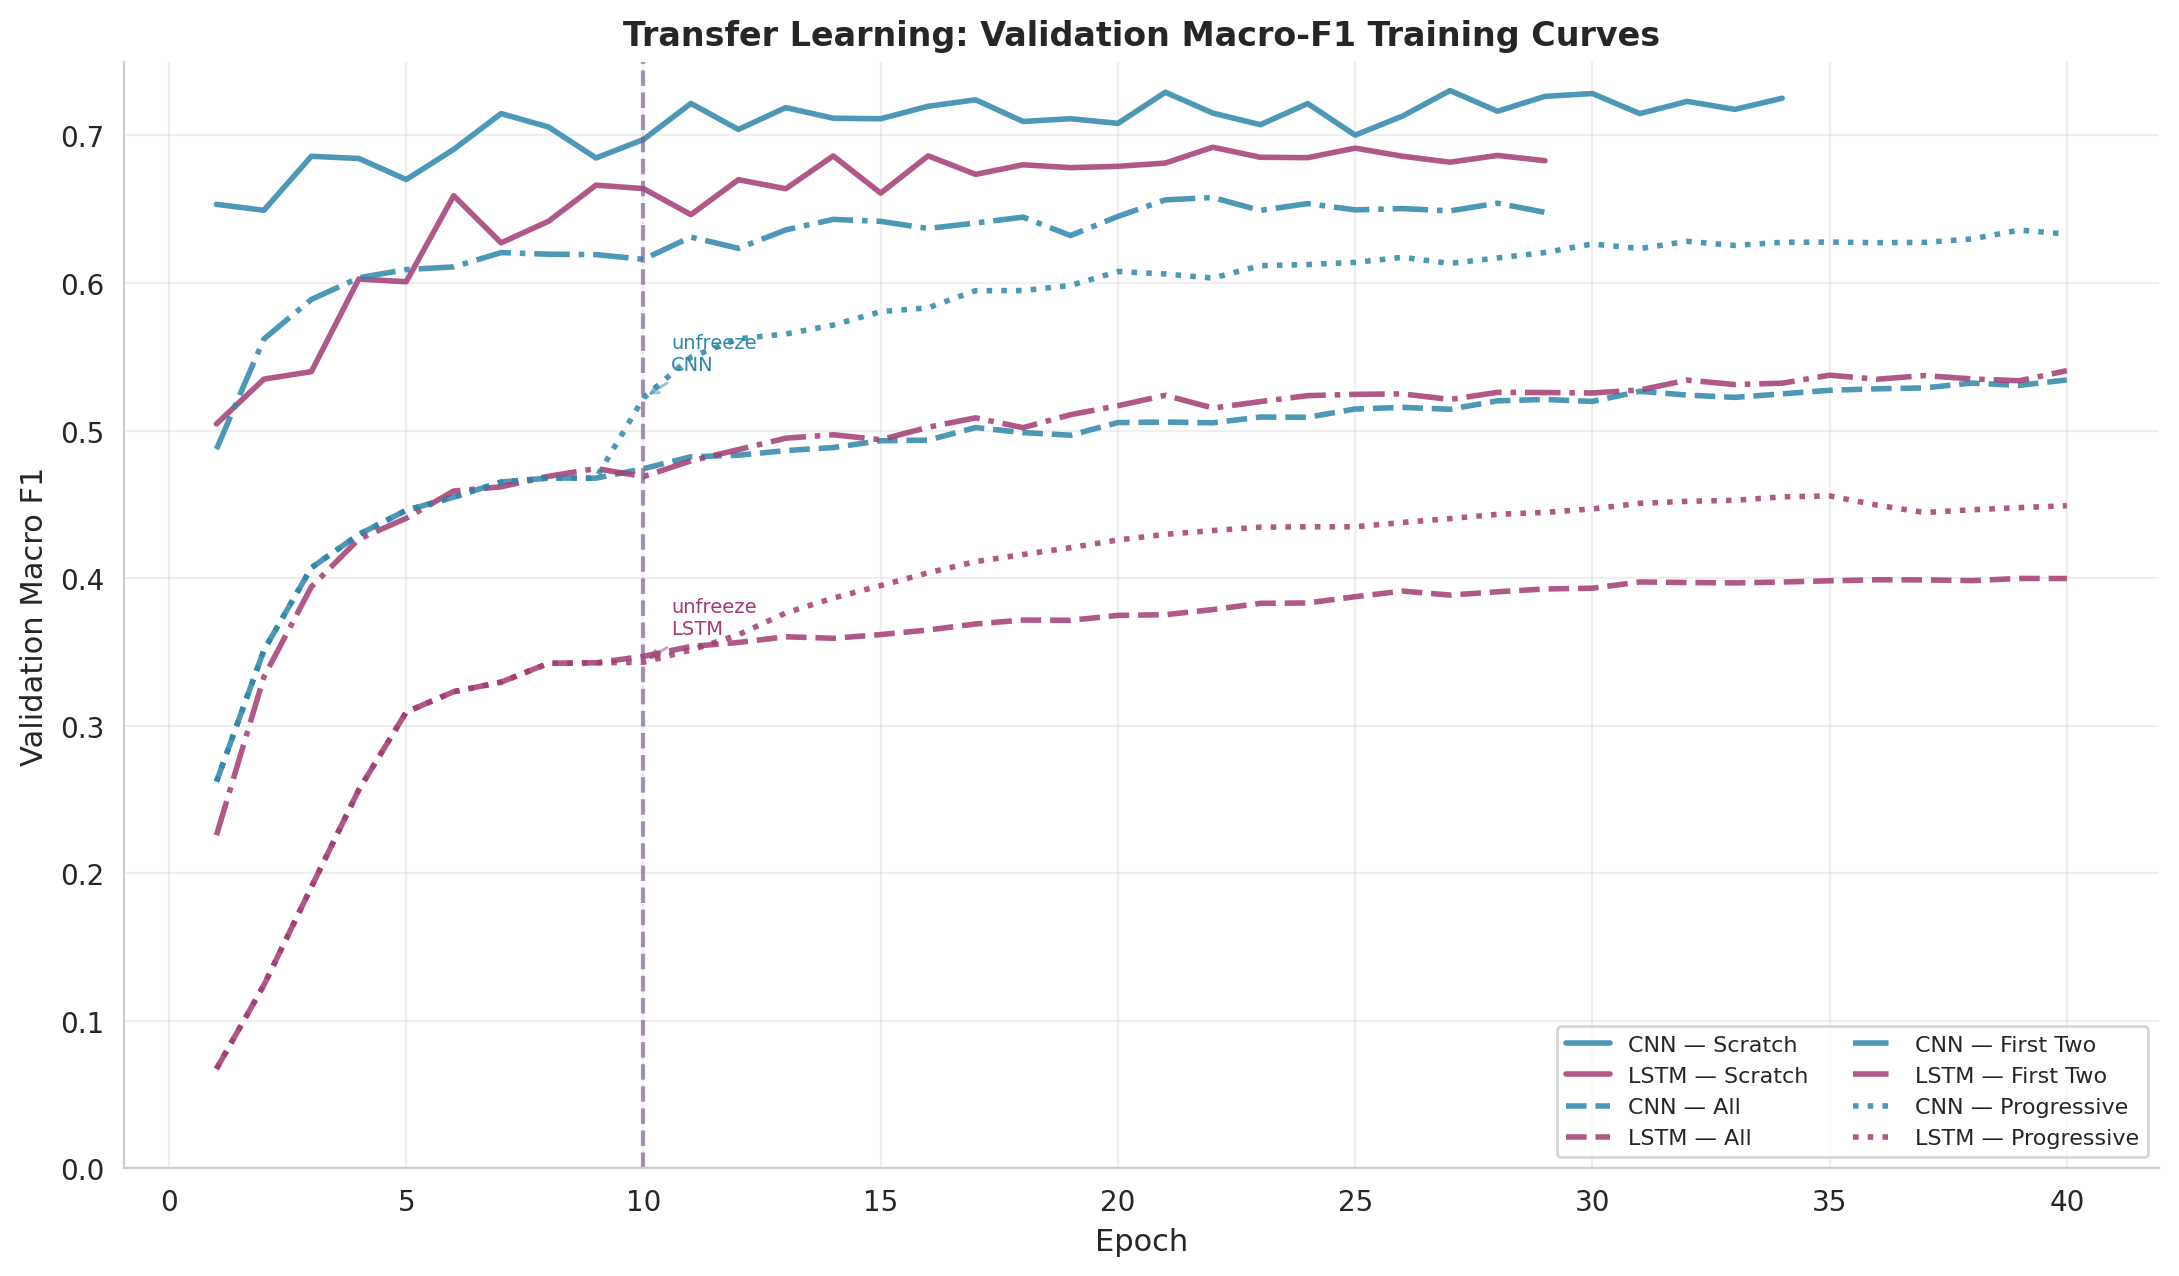
\includegraphics[width=0.98\linewidth]{figures/fig_transfer_curves.png}
  \caption{\textbf{Validation macro-F1 curves for all transfer configurations.}
  Watch-only scratch models (solid lines) plateau highest.
  Progressive runs (dotted lines) show a small uptick after the unfreeze annotation at epoch 10, but never recover to scratch levels.
  \label{fig:transfer-curves}}
\end{figure}

\subsubsection{Analysis: Negative Transfer}

The dominant finding is \textbf{negative transfer}: every pretrained configuration underperforms its from-scratch counterpart.
For CNN, the accuracy drops are $-13.3$ percentage points (frozen), $-5.8$ (partial), and $-6.3$ (progressive).
For LSTM the drops are even more severe: $-26.2$, $-13.7$, and $-18.3$ points respectively.
The frozen strategy is consistently the worst, confirming that UCI HAR features are not directly reusable as a fixed representation for our 18-class problem.

Partial fine-tuning is the ``least bad'' strategy for both architectures, suggesting that the bottom layers of the UCI HAR encoder learned motion primitives that are at least partially adaptable, while the top layers are too task-specific.
Progressive unfreezing at epoch 10 produces a visible but insufficient recovery in validation F1 (Figure~\ref{fig:transfer-curves}), and the test-time gap to scratch remains large.

We attribute the negative transfer to a \textbf{domain gap} rather than a bug in the protocol.
UCI HAR activities are coarse-grained daily motions (walking, sitting, standing) recorded from a waist-mounted phone, whereas our dataset contains 18 finer-grained activity codes (A--S) recorded from both wrist and pocket.
The learned filters that discriminate ``walking upstairs'' from ``sitting'' are not the same filters needed to disambiguate our finer activity classes.
This finding is consistent with the broader transfer-learning literature: pretraining helps only when the source and target domains share relevant low-level structure.

\subsection{Training Dynamics}

Figure~\ref{fig:training-curves} shows validation-macro-F1 learning curves for all nine runs.
Watch-only models train for the longest (22--39 epochs) and reach the highest plateaus.
Fusion and phone models converge much earlier (1--16 epochs) at substantially lower levels, confirming that poor performance is not due to insufficient training but to weak or noisy input signal.

\begin{figure}[htb!]
  \centering
  \includegraphics[width=0.98\linewidth]{drive-download-figures/fig2_training_curves_grid.png}
  \caption{\textbf{Validation macro-F1 curves across all nine runs.}
  Watch-only models train longer and plateau higher; phone and fusion models stop early with low validation F1.}
  \label{fig:training-curves}
\end{figure}

\subsection{Headline Comparison: Deep vs Classical vs Contrastive}

Table~\ref{tab:main-results} places the best deep models in context against classical ML and contrastive probes.
The CNN watch baseline (0.6447) outperforms Random Forest (0.6021), the strongest classical model, by 4.3 percentage points.
The contrastive watch probe (0.5831) trails the supervised CNN by 6.2 points but remains competitive with the ANN watch baseline.

\begin{table}[httb!] \scriptsize
\centering
    \begin{tabularx}{0.98\textwidth}{ l  l  c  c  c  c  c }
        \toprule
        \textbf{Method} & \textbf{Input} & \textbf{Labels} & \textbf{Prec.} & \textbf{Recall} & \textbf{Acc.} & \textbf{Macro F1} \\
        \midrule
        \rowcolor{LightBlue} CNN watch baseline           & watch raw                        & 100\% & 0.6773 & 0.6447 & 0.6447 & 0.6471 \\
        LSTM watch baseline          & watch raw                        & 100\% & 0.6485 & 0.6127 & 0.6127 & 0.6117 \\
        \rowcolor{LightBlue} ANN watch baseline           & watch raw                        & 100\% & 0.6291 & 0.5942 & 0.5942 & 0.5930 \\
        Supervised watch baseline    & watch raw                        & 10\%  & 0.6308 & 0.6155 & 0.6155 & 0.6078 \\
        \rowcolor{LightBlue} Random Forest                & handcrafted 84-D                 & 100\% & 0.6221 & 0.6021 & 0.6021 & 0.5838 \\
        Contrastive watch probe      & watch emb.                       & 100\% & 0.6033 & 0.5831 & 0.5831 & 0.5777 \\
        \rowcolor{LightBlue} Contrastive watch probe      & watch emb.                       & 10\%  & 0.5762 & 0.5647 & 0.5647 & 0.5556 \\
        Contrastive paired probe     & phone+watch emb.                 & 100\% & 0.5138 & 0.4861 & 0.4861 & 0.4707 \\
        \rowcolor{LightBlue} Contrastive paired probe     & phone+watch emb.                 & 10\%  & 0.5066 & 0.4795 & 0.4795 & 0.4658 \\
        Contrastive phone probe      & phone emb.                       & 100\% & 0.1805 & 0.1692 & 0.1692 & 0.1540 \\
        \rowcolor{LightBlue} Contrastive phone probe      & phone emb.                       & 10\%  & 0.1908 & 0.1793 & 0.1793 & 0.1603 \\
        \bottomrule
    \end{tabularx}
    \caption{\textbf{Headline results across all model tiers.}
    The CNN watch baseline is the strongest deep model in the current artifact set.
    As in Table~\ref{tab:classical-results}, macro recall equals accuracy because the test split is exactly class-balanced.
    \label{tab:main-results}}
\end{table}

\subsection{Interpretation}

\subsubsection{Architecture Hierarchy on Watch}

The CNN outperforms both LSTM and ANN on watch-only input.
We attribute this to the CNN's inductive bias: local temporal convolutional filters naturally capture motion-pattern primitives (e.g., stroke cycles, gait phases) that are discriminative for activity classes, while adaptive average pooling aggregates these local features into a fixed-size representation.
The LSTM, despite its temporal modeling capacity, underperforms the CNN; mean-pooling over all time steps may lose fine-grained temporal structure that the CNN's hierarchical subsampling preserves.
The ANN, lacking any temporal structure beyond the flattened vector ordering, performs worst among the three, confirming that raw-window flattening is insufficient for this task.

\subsubsection{Device Asymmetry is Architecture-Independent}

The most striking finding is that phone-only performance is near-random ($\sim$18\%) across \emph{all} architectures (CNN: 18.2\%, LSTM: 19.5\%, ANN: 18.1\%).
This rules out the hypothesis that phone data could be exploited with a better architecture; the signal is fundamentally weak for subject-disjoint classification under the current preprocessing.

Fusion performance is also consistently worse than watch-only: CNN drops from 64.5\% to 50.0\%, LSTM from 61.3\% to 38.0\%, and ANN from 59.4\% to 38.7\%.
This confirms that phone channels add noise that no tested architecture successfully suppresses.
Figure~\ref{fig:accuracy-by-channel} makes this degradation visually explicit.

\begin{figure}[htb!]
  \centering
  \includegraphics[width=0.72\linewidth]{drive-download-figures/fig6_accuracy_by_channel.png}
  \caption{\textbf{Accuracy by channel mode across architectures.}
  Every architecture degrades when phone data is included, with CNN showing the smallest absolute drop on fusion but still losing 14.5 points relative to watch-only.}
  \label{fig:accuracy-by-channel}
\end{figure}

\subsubsection{Error Patterns}

Figure~\ref{fig:confusion-matrices-grid} shows confusion matrices for all nine runs.
The watch-only CNN exhibits the sharpest diagonal, while phone-only matrices are nearly uniform (consistent with chance performance).
The error structure is architecture-agnostic: classes B, O, and P remain easy across all models, while F, I, J, K, and L remain difficult.

\begin{figure}[htb!]
  \centering
  \includegraphics[width=0.98\linewidth]{drive-download-figures/fig3_confusion_matrices_grid.png}
  \caption{\textbf{Confusion matrices for all nine model--channel combinations.}
  Watch-only models (top row) show strong diagonal structure; phone-only models (bottom row) are near-uniform.}
  \label{fig:confusion-matrices-grid}
\end{figure}

\subsection{Per-Class F1 Comparison}

Figure~\ref{fig:per-class-f1-all} extends the per-class analysis to all three architectures on watch-only input.
CNN leads on the majority of classes, with the largest margins on the difficult classes (F, I, J, K, L).
This suggests that the CNN's local filtering is particularly effective at disambiguating subtle motion patterns that confuse the LSTM and ANN.

\begin{figure}[htb!]
  \centering
  \includegraphics[width=0.98\linewidth]{drive-download-figures/fig4_per_class_f1_comparison.png}
  \caption{\textbf{Per-class F1 comparison across CNN, LSTM, and ANN on watch-only input.}
  CNN dominates on most classes, especially the difficult ones (F, I, J, K, L).}
  \label{fig:per-class-f1-all}
\end{figure}

\subsection{Subject Generalization}

Figure~\ref{fig:per-subject-heatmap} shows per-subject test accuracy for the three watch-only models.
Subject-to-subject variation is substantial (ranging from $\sim$45\% to $\sim$80\%), but the relative ranking of CNN~$>$~LSTM~$>$~ANN is stable across nearly all subjects.
This consistency reinforces the architectural conclusion: the CNN's stronger performance is not driven by a few easy subjects but generalizes across the held-out population.

\begin{figure}[htb!]
  \centering
  \includegraphics[width=0.98\linewidth]{drive-download-figures/fig5_per_subject_accuracy_heatmap.png}
  \caption{\textbf{Per-subject accuracy heatmap for watch-only models.}
  CNN $>$ LSTM $>$ ANN holds for almost every subject; absolute accuracy varies widely across subjects.}
  \label{fig:per-subject-heatmap}
\end{figure}

\subsection{ROC / AUC}

Figure~\ref{fig:roc-curves} plots macro one-vs-rest ROC curves for the CNN watch baseline and the contrastive watch probe.
Both curves lie well above the diagonal, but the CNN achieves stronger aggregate discrimination, consistent with its higher test accuracy and macro F1.

\begin{figure}[htb!]
  \centering
  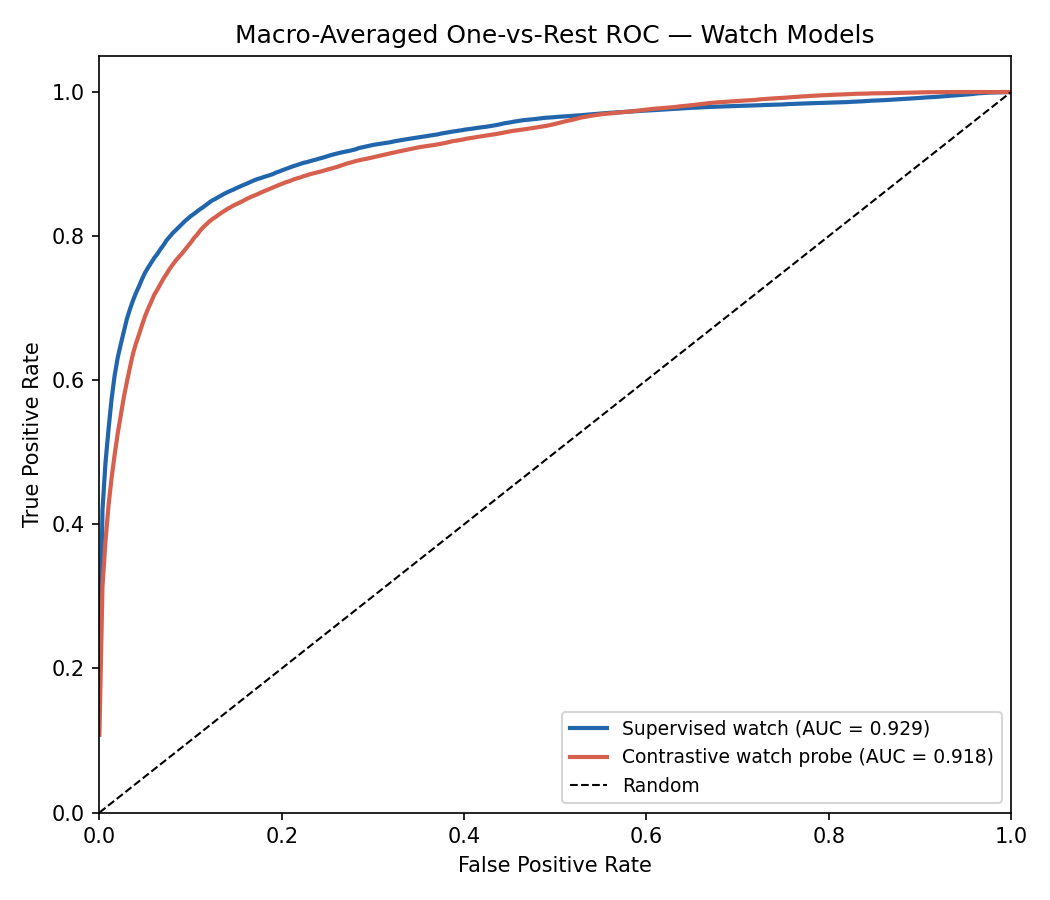
\includegraphics[width=0.72\linewidth]{figures/roc_auc_watch_vs_ssl.png}
  \caption{\textbf{Macro one-vs-rest ROC curves for the watch-first benchmark comparison.}
  CNN watch baseline (blue) and contrastive watch probe (red).}
  \label{fig:roc-curves}
\end{figure}

\section{Conclusion}
\label{sec:CONCLUSIONS}

This project delivers a complete end-to-end pipeline from raw phone and watch inertial files to subject-disjoint quantitative evaluation.
The main engineering contribution is a segment-aware alignment and resampling pipeline that converts heterogeneous raw streams into stable multimodal windows.

The main empirical result is that the supervised watch-only CNN baseline is the best deep model under subject-disjoint evaluation, reaching 64.47\% accuracy and 0.6471 macro F1.
The full architecture sweep shows that CNN $>$ LSTM $>$ ANN on watch-only input, and that this ordering is stable across individual subjects.
A critical complementary finding is that device asymmetry is architecture-independent: phone-only performance is near-random ($\sim$18\%) for CNN, LSTM, and ANN alike, and fusion degrades all three architectures relative to watch-only.
This suggests that the phone signal is fundamentally weak for subject-disjoint classification under the current preprocessing, rather than merely requiring a better model.

The five-tier evaluation provides a useful ladder of baselines: classical models on handcrafted features establish an interpretable reference point (Random Forest: 60.21\%), supervised deep learning provides the strongest benchmark (CNN watch: 64.47\%), the architecture sweep characterizes the value of temporal modeling (CNN vs LSTM vs ANN), contrastive pretraining shows partial gains over naive fusion without yet delivering the best overall result (watch probe: 58.31\%), and transfer learning from UCI HAR reveals that negative transfer can occur when the source and target domains are too dissimilar.

\textbf{Future work.}
Three directions remain open after the current artifact set.
First, \textbf{transfer learning with a closer domain}: we explored fine-tuning encoders pretrained on UCI HAR and observed negative transfer across all freezing strategies.
Future work could investigate whether a more domain-similar pretraining corpus (e.g., another wrist-based HAR dataset with finer-grained activities) would yield positive transfer, or whether domain-adversarial training could bridge the gap between pretraining and target domains.
Second, \textbf{phone signal diagnosis}: understanding why phone-only accuracy is near-random---whether due to sensor placement, orientation variability, or preprocessing---could unlock genuinely multimodal fusion.
Third, \textbf{advanced fusion}: gated or attention-weighted fusion that learns to dynamically downweight phone features may outperform the simple concatenation used here.

\section*{Member Contributions}

Krishna Mula and Yash Khairnar contributed equally to this project.
Work was shared jointly across dataset exploration, preprocessing and windowing, feature extraction, modeling and evaluation, figure generation, and report writing.

\section*{Availability of Data and Software}
\label{sec:AVAILABILITY}

Raw inertial files are stored in \texttt{data/}.
Derived window caches are in \texttt{artifacts/windows/}, supervised outputs in \texttt{artifacts/baseline/}, contrastive outputs in \texttt{artifacts/contrastive/}, and probe outputs in \texttt{artifacts/probes/}.
Training and evaluation code is under \texttt{src/}; the execution workflow is documented in \texttt{docs/phase2\_runbook.md}.
Before public release, redistribution rights for the raw dataset should be confirmed.

\footnotesize
\renewcommand{\refname}{}
\bibliographystyle{unsrt}
\bibliography{bibliography}
\normalsize

\end{document}
